\documentclass{article}

\usepackage[margin=1in]{geometry} 
\usepackage[fleqn]{mathtools}
\usepackage{amsmath,amsthm,amssymb}
\DeclareMathOperator*{\argmax}{argmax} % thin space, limits underneath in displays
\DeclareMathOperator*{\argmin}{argmin} % thin space, limits underneath in displays
\usepackage{graphicx}
\usepackage[toc,page]{appendix}
\usepackage[square,sort,comma,numbers]{natbib}
\bibliographystyle{acm} %acm, abbrv, ieeetr, plain, unsrt plainnat
\usepackage{listings}
\usepackage{color}
\usepackage{hyperref}
\usepackage{bm}
\usepackage{bbm}
\usepackage{pdfpages}

\newcommand{\E}{\mathbb{E}}
\newcommand{\V}{\mathrm{V}}
\newcommand{\N}{\mathcal{N}}
\newcommand{\R}{\mathbb{R}} 
\newcommand{\1}{\mathbbm{1}}


\title{Economics 631 IO - Fall 2019\\Problem Set 3}
\author{Nathan Mather and Tyler Radler}
\date{\today}

\begin{document}
\maketitle

\section{Production Function Estimation}

\subsection{Summary Statistics}

\begin{center}
	\centering
	\textbf{Summary Statistics -- Mean and Variance}\par\medskip
	\scalebox{1}{
		% latex table generated in R 3.6.1 by xtable 1.8-4 package
% Mon Dec 02 11:06:07 2019
\begin{tabular}{lrrrrrr}
  \hline
Variable & Full Mean & Bal. Mean & Tstat & Full VAR & Bal. VAR & Fstat \\ 
  \hline
ldsal & 5.67 & 6.91 & -17.15 & 3.84 & 3.38 & 1.14 \\ 
  lemp & 1.26 & 2.41 & -17.94 & 3.15 & 2.63 & 1.20 \\ 
  ldnpt & 4.47 & 5.92 & -17.81 & 4.91 & 4.23 & 1.16 \\ 
  ldrst & 3.40 & 4.89 & -19.60 & 4.12 & 3.72 & 1.11 \\ 
  ldrnd & 1.79 & 3.22 & -18.42 & 4.21 & 3.98 & 1.06 \\ 
  ldinv & 2.67 & 4.07 & -17.27 & 4.71 & 4.22 & 1.12 \\ 
   \hline
\end{tabular}

	}
\end{center}

\begin{center}
	\centering
	\textbf{Summary Statistics -- Min and Max}\par\medskip
	\scalebox{1}{
		% latex table generated in R 3.6.1 by xtable 1.8-4 package
% Mon Dec 02 11:06:07 2019
\begin{tabular}{lrrrrrr}
  \hline
Variable & Full Mean & Bal. Mean & Tstat & Full VAR & Bal. VAR & Fstat \\ 
  \hline
ldsal & 5.67 & 6.91 & -17.15 & 3.84 & 3.38 & 1.14 \\ 
  lemp & 1.26 & 2.41 & -17.94 & 3.15 & 2.63 & 1.20 \\ 
  ldnpt & 4.47 & 5.92 & -17.81 & 4.91 & 4.23 & 1.16 \\ 
  ldrst & 3.40 & 4.89 & -19.60 & 4.12 & 3.72 & 1.11 \\ 
  ldrnd & 1.79 & 3.22 & -18.42 & 4.21 & 3.98 & 1.06 \\ 
  ldinv & 2.67 & 4.07 & -17.27 & 4.71 & 4.22 & 1.12 \\ 
   \hline
\end{tabular}

	}
\end{center}

There appear to be significant differences between the full sample and the balanced panel. In particular, the mean of each of the variables in the balanced panel is higher than that in the full sample, suggesting that firms which stay in the sample for the entire time period are generally larger and invest more. This makes sense, as we'd expect firms who eventually exit the market to be the least productive firms, and therefore produce and invest less. The full panel also has higher variance than the balanced panel, which would make sense as we are including firms with generally lower values relative to the balanced panel, which should increase the variance. The minimum values are similarly lower in the full sample relative to the balanced panel, and the maximum values all appear in the balanced panel. Broadly it seems clear that the balanced panel is a selected sample.

\subsection{Production Function Estimation}

\begin{center}
	\centering
	\textbf{Production Function Coefficients}\par\medskip
	\scalebox{1}{
		% latex table generated in R 3.6.1 by xtable 1.8-4 package
% Mon Dec 02 10:50:32 2019
\begin{tabular}{lrrr}
  \hline
parm & statistic & bias & std.error \\ 
  \hline
B\_0 & 0.97 & 0.05 & 0.05 \\ 
  L & 0.48 & 0.05 & 0.04 \\ 
  K & 0.43 & -0.03 & 0.02 \\ 
  RD & 0.05 & -0.01 & 0.01 \\ 
  P & 1.00 & 0.00 & 0.00 \\ 
   \hline
\end{tabular}

	}
\end{center}

The production function estimates are reported above, with the bootstrapped standard errors reported on the right. A few things -- we interpreted ``ignoring the selection issue'' to mean using the balanced panel and not worrying about the fact this panel should consist of firms with the highest productivity. Estimates using the full panel were quite similar. In our reported results we stratified the bootstrap at the firm level, but have also experimented with iid bootstrapping at the observation level. Our concern with the latter was figuring out how to deal with the lagged variables. Realistically the answer is probably to block-bootstrap but we decided to stratify at the firm level as a middle ground.

In terms of the coefficients, a few things to note are that the production function is DRS, but only weakly so -- in fact, the coefficients sum to .96, which is much closer to 1 than we expected. We weren't sure what to make of the $\rho$ being so close to 1. This appears to be the case regardless of which sample we use. This means that any productivity shock is basically entirely persistent. If this were the case we could potentially treat the productivity shocks as a firm-specific fixed effect we could get rid of by differencing. 

$$\E[w_{it} - w_{it-1}]= \E[w_{it-1}*\rho +\xi_{it} - w_{it-1}] \approx \E[\xi_{it}] = 0$$

This seems weird, although this potentially points to an error in our code.

%------------------------------------------------
% APPENDIX
%------------------------------------------------



\section{Appendix}
\subsection{R Code}

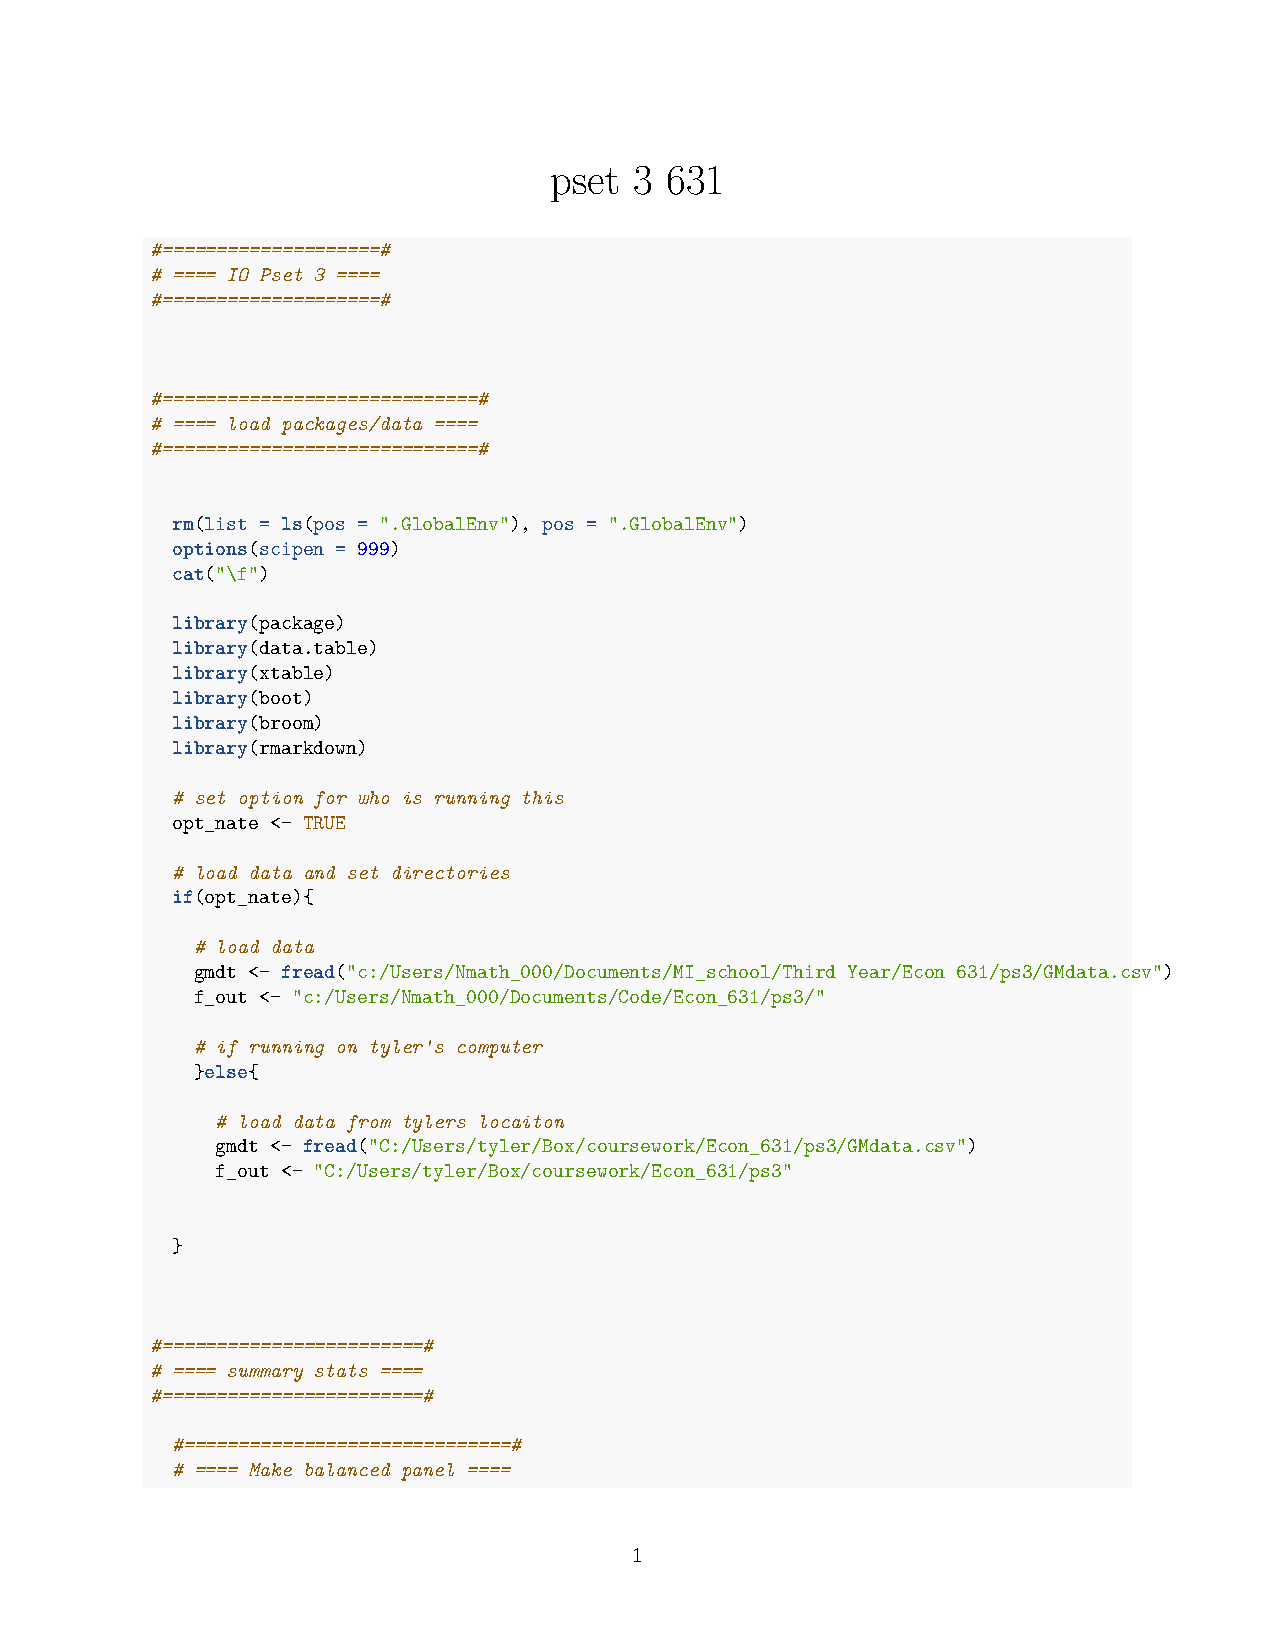
\includepdf[page=-]{assignment_3_r_code_pdf.pdf}





\end{document}
